%standard 4.1

%start_of_questions

%new_question
%%%%%%%%%%%%%%%%%%%%%
	% Problem 1
	% Difficulty: 1
%%%%%%%%%%%%%%%%%%%%%
	\item  
		%https://edabit.com/challenge/Ay9wPrqRJnBmvbFmi
		Ask the user for two integers named \textit{larger} and \textit{smaller}.  
		Determine (and output) how many times larger can be halved while still be 
		greater than smaller.
		
		Examples:
		\begin{itemize}
			\item if \textit{larger} = 1324 and  \textit{smaller} = 98, the result should be 3 since
				1324 $\rightarrow$ 662 $\rightarrow$ 331 $\rightarrow$ 165.5
			\item if \textit{larger} = 624 and  \textit{smaller} = 8, the result should be 6 since\\
				\tab 624 $\rightarrow$ 312 $\rightarrow$ 156 $\rightarrow$ 78 $\rightarrow$ 39 
				$\rightarrow$ 19.5 $\rightarrow$ 9.75)
		\end{itemize}


%new_question
%%%%%%%%%%%%%%%%%%%%%
	% Problem 2
	% Difficulty: 1
%%%%%%%%%%%%%%%%%%%%%
	\item  
		Write a program that asks the user for a word and then, \underline{using a loop}, 
		prints every other letter of the word starting with the second letter.

		Examples:
		\begin{itemize}
			\item if user\_word = \csq{counterattack}, the result should be \csq{oneatc}
			\item if user\_word = \csq{banana sunday}, the result should be \csq{aaasna}
		\end{itemize}


%new_question
%%%%%%%%%%%%%%%%%%%%%
	% Problem 3
	% Difficulty: 1
%%%%%%%%%%%%%%%%%%%%%
	\item  
		Using a loop, write a program that prints every even number 
		between 37 and 1050 (inclusively).


%new_question
%%%%%%%%%%%%%%%%%%%%%
	% Problem 5
	% Difficulty: 1
%%%%%%%%%%%%%%%%%%%%%
	\item  
		Using a loop, write code to calculate the sum of all odd numbers between 50 and 517. 
		Print the result.


%new_question
%%%%%%%%%%%%%%%%%%%%%
	% Problem 8
	% Difficulty: 1
%%%%%%%%%%%%%%%%%%%%%
	\item  
		%https://edabit.com/challenge/6Pf5GGG6HnzbB95gf
		Write code that asks the user for an integer and then prints each number that is a 
		factor of the input.
	
		For example, \\ \ \hfill
		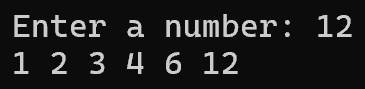
\includegraphics[height = .35in]{./imgs/factors1.PNG} \hfill  
		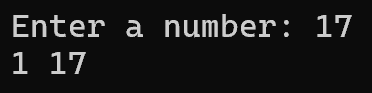
\includegraphics[height = .35in]{./imgs/factors2.PNG} \hfill  
		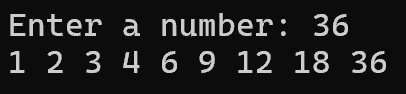
\includegraphics[height = .35in]{./imgs/factors3.PNG} \hfill \


%new_question
%%%%%%%%%%%%%%%%%%%%%
	% Problem 11
	% Difficulty: 1
%%%%%%%%%%%%%%%%%%%%%
	\item  
		%https://edabit.com/challenge/aqDGJxTYCx7XWyPKc
		Write a program that asks the user for an integer.  Calculate (and then print) the 
		sum of all square numbers up to and including the user's number.

		For example, 
		\begin{itemize}
			\item if user\_number = 3, the result should be 14 since $1^2 + 2^2 + 3^2 = 14$.
			\item if user\_number = 8, the result should be $1^2+2^2+3^2+4^2+5^2+6^2+7^2+8^2=204$.
		\end{itemize}

%end_of_questions

